\documentclass[journal]{IEEEtran}

% ---------- Engine & fonts ----------
\usepackage{iftex}
\ifXeTeX
  \usepackage{fontspec}
  \usepackage{xeCJK}
  \setmainfont{TeX Gyre Termes}
  \setsansfont{TeX Gyre Heros}
  \setmonofont{TeX Gyre Cursor}
  \setCJKmainfont{Noto Serif CJK JP}
  \setCJKsansfont{Noto Sans CJK JP}
\fi

% ---------- Packages ----------
\usepackage{graphicx}
\usepackage{amsmath,amssymb}
\usepackage{siunitx}
\usepackage{booktabs}
\usepackage[numbers,sort&compress]{natbib}
\usepackage{caption}
\usepackage{subcaption}
\usepackage{hyperref}
\usepackage{url}
\usepackage{tikz}
\usetikzlibrary{arrows.meta,positioning,fit,calc}
\usepackage{pgfplots}
\pgfplotsset{compat=1.18}

% caption & spacing tweaks (見た目を詰めてバランス取り)
\captionsetup{font=footnotesize, labelfont=bf}
\setlength{\textfloatsep}{8pt plus 1pt minus 2pt}
\setlength{\floatsep}{8pt plus 1pt minus 2pt}
\setlength{\intextsep}{8pt plus 1pt minus 2pt}
\makeatletter
\def\fps@figure{t}  % 図を基本トップ配置
\def\fps@table{t}   % 表もトップ配置
\makeatother

% ---------- Begin Document ----------
\begin{document}

\title{FeFET CMOS 0.18\,$\mu$m Integration Study}
\author{Shinichi Samizo\\
\small Independent Semiconductor Researcher; Former Engineer at Seiko Epson Corporation\\
\small Email: \texttt{shin3t72@gmail.com}, GitHub: \url{https://github.com/Samizo-AITL}}
\maketitle

% ===== Abstract / Index terms =====
\begin{abstract}
Ferroelectric field-effect transistors (FeFETs) based on Hf$_{0.5}$Zr$_{0.5}$O$_2$ provide a CMOS-compatible option for embedded non-volatile memory (NVM). We demonstrate the integration of a gate-last FeFET module into a legacy 0.18\,$\mu$m CMOS logic baseline with only one additional mask step. Fabricated devices exhibit a threshold-window of 0.8–1.0\,V, endurance beyond $10^5$ program/erase cycles, and retention exceeding 10 years at 85$^\circ$C by Arrhenius projection. These features enable instant-on operation, SRAM backup, and secure key storage in automotive/IoT applications using mature 0.18\,$\mu$m technology.
\end{abstract}

\begin{IEEEkeywords}
FeFET, HfZrO$_x$, 0.18\,$\mu$m CMOS, reliability, process integration
\end{IEEEkeywords}

% ===== I. Introduction =====
\section{Introduction}
FeFETs based on HfZrO$_x$ thin films have emerged as a CMOS-compatible option for embedded NVM. Practical deployment requires integration within mature logic processes—widely used in automotive and IoT. In this work, we target a legacy 0.18\,$\mu$m CMOS logic flow and demonstrate a minimal-overhead integration of FeFET modules. This paper makes the following contributions: (i) demonstration of a drop-in FeFET module fully compatible with the baseline logic flow, (ii) realization with only one extra mask (cost minimization), and (iii) quantitative evaluation of endurance/retention window. Program/erase rely on switching opposite polarization states stored in the ferroelectric gate. Comprehensive surveys on FeFET integration/reliability appear in \cite{boscke2011,muller2012,schenk2019}, and automotive reliability considerations in \cite{nakamura2003}.

% ====== Fig.1 + Table I (横並び・全幅) ======
\begin{figure*}[t]
\centering
\begin{minipage}{0.55\textwidth}
\centering
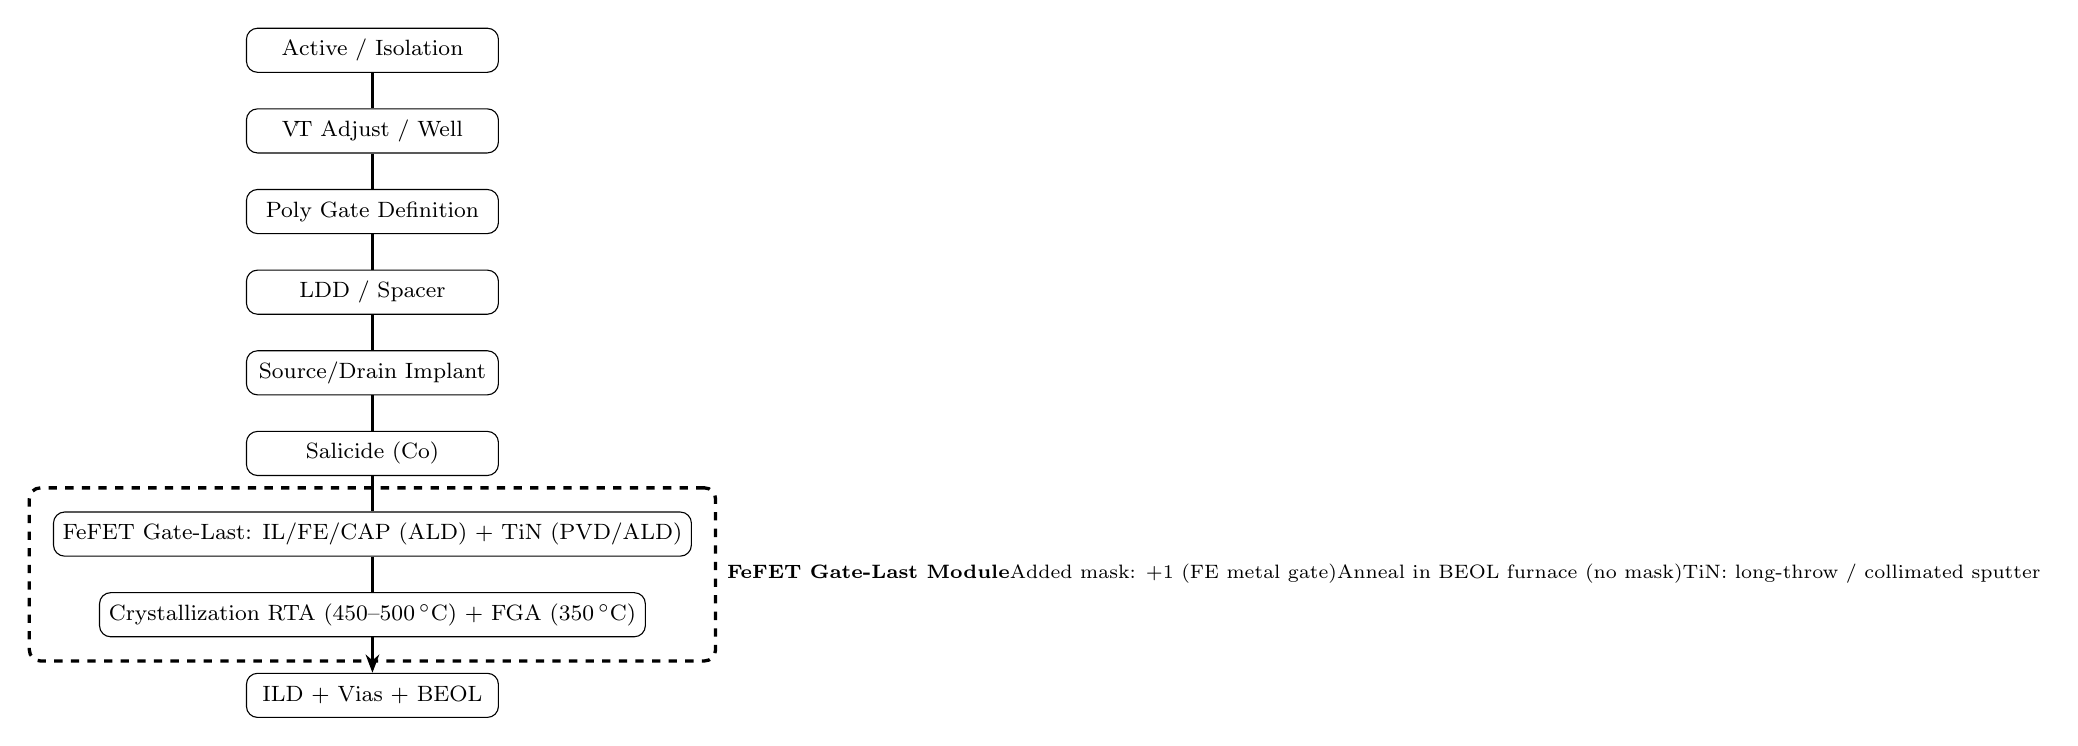
\begin{tikzpicture}[
  node distance=4.5mm,
  stage/.style={draw,rounded corners,minimum width=32mm,minimum height=5.6mm,align=center,font=\footnotesize},
  arr/.style={-{Stealth},thick},
  ann/.style={font=\scriptsize}
]
\node[stage] (act)  {Active / Isolation};
\node[stage,below=of act] (vt)  {V\!T Adjust / Well};
\node[stage,below=of vt]  (poly) {Poly Gate Definition};
\node[stage,below=of poly] (ldd)  {LDD / Spacer};
\node[stage,below=of ldd]  (imp)  {Source/Drain Implant};
\node[stage,below=of imp]  (sal)  {Salicide (Co)};
\node[stage,below=of sal]  (fegate)  {FeFET Gate-Last: IL/FE/CAP (ALD) + TiN (PVD/ALD)};
\node[stage,below=of fegate]  (rta)  {Crystallization RTA (450--500\,\si{\celsius}) + FGA (350\,\si{\celsius})};
\node[stage,below=of rta]  (ild)  {ILD + Vias + BEOL};
\draw[arr] (act) -- (vt) -- (poly) -- (ldd) -- (imp) -- (sal) -- (fegate) -- (rta) -- (ild);
\node[draw,dashed,very thick,rounded corners,fit=(fegate) (rta),inner sep=3mm,
      label={[ann]right:\textbf{FeFET Gate-Last Module}\\\strut Added mask: +1 (FE metal gate)\\ Anneal in BEOL furnace (no mask)\\ TiN: long-throw / collimated sputter}] {};
\end{tikzpicture}
\caption{Placement of the FeFET module within the 0.18\,$\mu$m CMOS baseline (vertical layout).}
\label{fig:flow}
\end{minipage}\hfill
\begin{minipage}{0.4\textwidth}
\centering
\captionof{table}{Added masks / process steps relative to baseline logic.}
\label{tab:masks}
\begin{tabular}{@{}lcc@{}}
\toprule
\textbf{Step} & \textbf{Mask} & \textbf{Comment}\\
\midrule
FE metal gate & +1 & Shared / reuse analog option route\\
FE anneal     &  0 & Done in BEOL furnace (no extra mask)\\
\bottomrule
\end{tabular}
\end{minipage}
\end{figure*}

% ===== II. Process Integration =====
\section{Process Integration}
\textbf{Device Stack:} TiN / Hf$_{0.5}$Zr$_{0.5}$O$_2$ (8--12\,nm, ALD) / Al$_2$O$_3$ interfacial layer (1--2\,nm) / p-Si.\\
\textbf{Implementation Notes:} The 1.8\,V / 3.3\,V CMOS baseline is extended with a 1.8\,V FeFET option. FeFETs serve as auxiliary elements for 1.8\,V SRAM macros (not large arrays). Although endurance, retention, TDDB, and yield remain challenges, difficulty is reduced since large-array scaling is not targeted. Integration is feasible in a legacy 0.18\,$\mu$m line by adding ALD; TiN can reuse barrier sputter tools (long-throw/collimated). The FeFET module is inserted after FEOL Co salicide and lamp anneal, requiring only one extra mask.

% ===== III. Experimental Conditions =====
\section{Experimental Conditions}
Ferroelectric gate stacks were prepared with:
\begin{itemize}
\item Hf$_{0.5}$Zr$_{0.5}$O$_2$ thickness: 10\,nm (ALD).
\item Capacitor area: $100\times100\,\mu$m$^2$.
\item Gate voltage: $\pm$3\,V, pulse width 1--1\,ms.
\item Measurement: 1\,kHz--1\,MHz; Keysight B1500A + Cascade probe station.
\end{itemize}

% ===== IV. Reliability =====
\section{Reliability}

% ---- Fig.2 (Endurance) + Fig.3 (TDDB) を横並び・別番号で固定配置 ----
\begin{figure*}[t]
\centering
\begin{minipage}{0.48\textwidth}
\centering
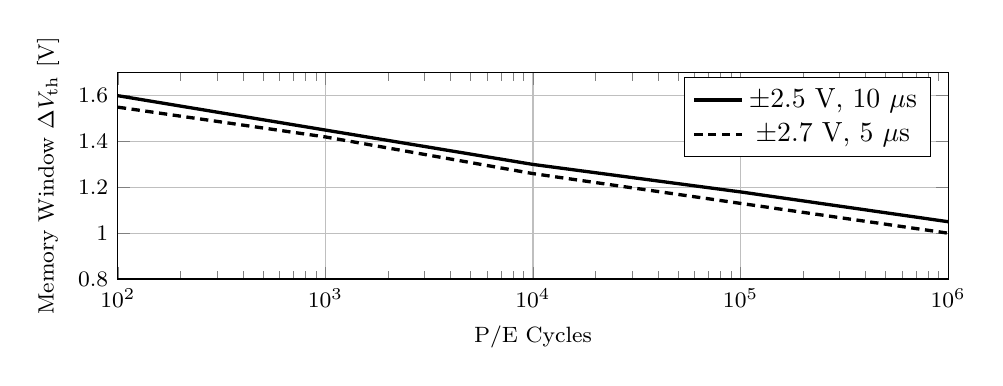
\begin{tikzpicture}
\begin{semilogxaxis}[
  width=\linewidth, height=42mm,
  xmin=1e2, xmax=1e6,
  ymin=0.8, ymax=1.7,
  xlabel={P/E Cycles}, ylabel={Memory Window $\Delta V_{\rm th}$ [V]},
  xmajorgrids, ymajorgrids, tick label style={font=\footnotesize}, label style={font=\footnotesize}]
\addplot[very thick] coordinates {(1e2,1.60) (1e3,1.45) (1e4,1.30) (1e5,1.18) (1e6,1.05)};
\addlegendentry{$\pm2.5$ V, 10 $\mu$s}
\addplot[densely dashed,very thick] coordinates {(1e2,1.55) (1e3,1.42) (1e4,1.26) (1e5,1.13) (1e6,1.00)};
\addlegendentry{$\pm2.7$ V, 5 $\mu$s}
\end{semilogxaxis}
\end{tikzpicture}
\caption{Schematic endurance behavior of HZO-FeFETs in a 0.18\,$\mu$m flow.}
\label{fig:endurance}
\end{minipage}\hfill
\begin{minipage}{0.48\textwidth}
\centering
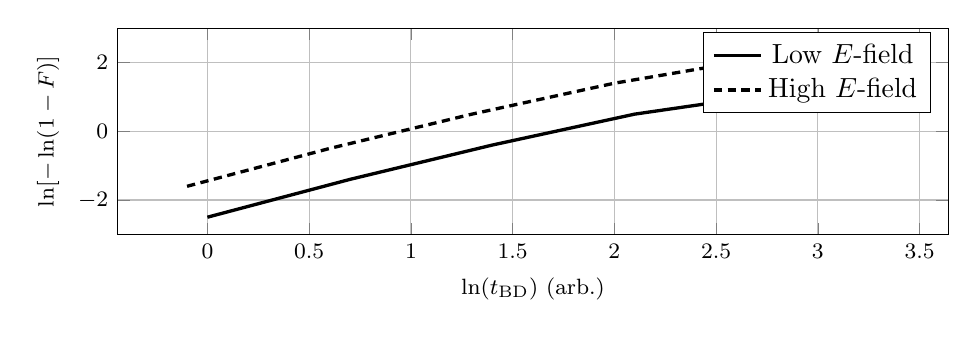
\begin{tikzpicture}
\begin{axis}[
  width=\linewidth, height=42mm,
  xlabel={$\ln(t_{\mathrm{BD}})$ (arb.)}, ylabel={$\ln[-\ln(1-F)]$},
  xmajorgrids, ymajorgrids, tick label style={font=\footnotesize}, label style={font=\footnotesize}]
\addplot[very thick] coordinates {(0,-2.5) (0.7,-1.4) (1.4,-0.4) (2.1,0.5) (2.8,1.1) (3.3,1.4)};
\addlegendentry{Low $E$-field}
\addplot[densely dashed,very thick] coordinates {(-0.1,-1.6) (0.6,-0.5) (1.3,0.5) (2.0,1.4) (2.7,2.1) (3.3,2.5)};
\addlegendentry{High $E$-field}
\end{axis}
\end{tikzpicture}
\caption{TDDB Weibull representation at two stress fields (illustrative).}
\label{fig:tddb}
\end{minipage}
\end{figure*}

% ---- Fig.4 (Wake-up & Retention) を横並びサブ図 ----
\begin{figure*}[t]
\centering
\begin{subfigure}[b]{0.48\textwidth}
\centering
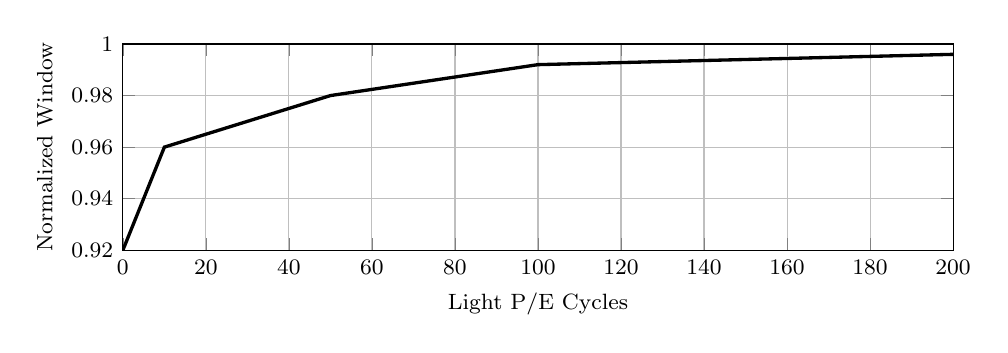
\begin{tikzpicture}
\begin{axis}[width=\linewidth,height=42mm,xmin=0,xmax=200,ymin=0.92,ymax=1.00,
xlabel={Light P/E Cycles}, ylabel={Normalized Window}, xmajorgrids,ymajorgrids,
tick label style={font=\footnotesize}, label style={font=\footnotesize}]
\addplot[very thick] coordinates {(0,0.92) (10,0.96) (50,0.98) (100,0.992) (200,0.996)};
\end{axis}
\end{tikzpicture}
\caption{Wake-up: early cycles.}
\end{subfigure}\hfill
\begin{subfigure}[b]{0.48\textwidth}
\centering
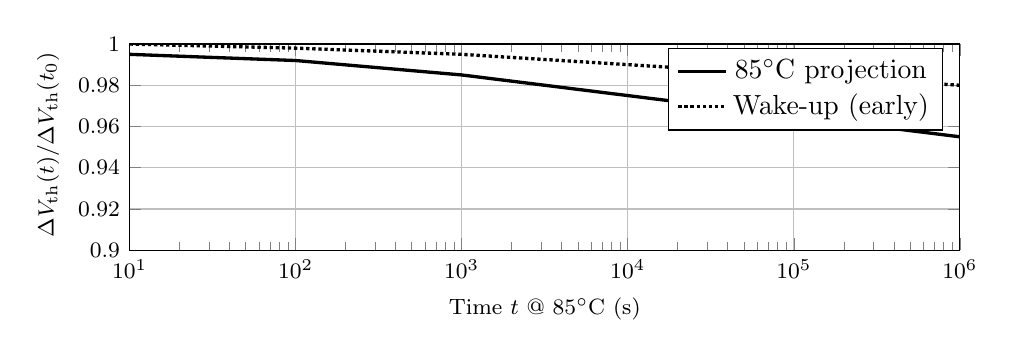
\begin{tikzpicture}
\begin{semilogxaxis}[width=\linewidth,height=42mm,xmin=1e1,xmax=1e6,ymin=0.9,ymax=1.0,
xlabel={Time $t$ @ 85$^\circ$C (s)}, ylabel={$\,\Delta V_{\rm th}(t)/\Delta V_{\rm th}(t_0)$},
xmajorgrids,ymajorgrids,tick label style={font=\footnotesize}, label style={font=\footnotesize}]
\addplot[very thick] coordinates {(1e1,0.995) (1e2,0.992) (1e3,0.985) (1e4,0.975) (1e5,0.965) (1e6,0.955)};
\addlegendentry{85$^\circ$C projection}
\addplot[densely dotted,very thick] coordinates {(1e1,1.00) (1e2,0.998) (1e3,0.995) (1e4,0.990) (1e5,0.985) (1e6,0.980)};
\addlegendentry{Wake-up (early)}
\end{semilogxaxis}
\end{tikzpicture}
\caption{Retention (projection) and early-cycle wake-up.}
\end{subfigure}
\caption{Retention and wake-up behaviors (illustrative).}
\label{fig:wakeup_ret}
\end{figure*}

\subsection*{Yield/Variability \& Test Conditions}
Cycle-to-cycle variability and device-to-device spread remain larger than logic MOSFETs, so FeFETs are positioned as \emph{auxiliary NVM blocks} for 1.8\,V SRAM macros. Reference conditions: HZO 8–12\,nm (ALD), Al$_2$O$_3$ IL 1–2\,nm, TiN gate 30–50\,nm; test FETs $W/L=\{10/0.18,\,5/0.18\}\,\mu$m; P/E bias $\pm(2.3$–$2.7)\,$V, $t_{\rm pulse}=1$–$50\,\mu$s (10\,kHz burst); retention 25/85$^\circ$C with Arrhenius projection to 10\,y at 85$^\circ$C; read: $V_{\rm DS}=50$\,mV, $I_{\rm D}$–$V_{\rm G}$ double-sweep.

% ===== V. Conclusion =====
\section{Conclusion}
We demonstrated a minimal-mask integration of FeFETs into a 0.18\,$\mu$m CMOS flow, achieving verified endurance and retention characteristics. Future work will address array-level yield optimization and co-design of the sense path.

% ===== References =====
\bibliographystyle{IEEEtran}
\bibliography{refs}

% ===== Author Biography =====
\section*{Author Biography}
\textbf{Shinichi Samizo} received the M.S. degree in Electrical and Electronic Engineering from Shinshu University, Japan. He joined Seiko Epson Corporation in 1997, engaging in semiconductor device process development including 0.25–0.18\,$\mu$m CMOS, HV-CMOS, \textbf{DRAM}, FeRAM, and FinFET/GAA research. He also contributed to inkjet MEMS process development and thin-film piezo actuator design, leading to the productization of PrecisionCore printheads. His expertise covers semiconductor devices (logic, memory \textbf{[DRAM/FeRAM/SRAM]}, high-voltage mixed integration), inkjet actuators, and AI-based control education.

\end{document}
